\documentclass[sigplan,10pt,manuscript,nonacm]{acmart}
%% Supplied to authors by publisher for64-bitra-ready submission;
%% use defaults fvalues,iew submission.
\settopmatter{printacmref=false}
% \acmConference[]aboutcmYear{}
\acmISBN{} % \acmISBN{978-x-xxxx-xxxx-x/YY/MM}
\acmDOI{} % \at solvingg us1145/nnnnnnn.nnnnnnn}
\startPage{1}

\usepackage{fancyhdr}


%% Copyright information
%% Supplied to authors (based on authors' rights management selection;
%% see authors.acm.org) by publisher for camera-ready submission;
%% use 'none' for review submission.
\setcopyright{none}
%\setcopyright{acmcopyright}
%\setcopyright{acmlicensed}
%\setcopyright{rightsretained}
%\copyrightyear{2018}           %% If different from \acmYear

%% Bibliography style
\bibliographystyle{ACM-Reference-Format}
\citestyle{acmnumeric}     %% For numeric citations

\usepackage[parfill]{parskip}

%\usepackage[table]{xcolor}
\PassOptionsToPackage{table}{xcolor}

\usepackage{colortbl}
\usepackage{amsmath}
\let\Bbbk\relax
\usepackage{color}
\usepackage{amssymb}
\usepackage{algorithmic}
%\usepackage{fancyhdr}
\usepackage{endnotes}
\usepackage{epsfig}
\usepackage{epstopdf}
\usepackage{caption}
\usepackage{subcaption}
\usepackage{url}
\usepackage{svg}
\usepackage{color}
\colorlet{shadecolor}{gray!30}
\usepackage{graphicx}
\usepackage{multirow}
\usepackage[breakable]{tcolorbox}

\usepackage{minted}
\usemintedstyle{manni}
\definecolor{CodeBG}{gray}{0.9}

\usepackage{pgfplots,tikz}
\usetikzlibrary{shapes, arrows.meta, positioning}

\usepackage{pgf-pie}
\usepackage{tikz-network}
\usetikzlibrary{arrows,automata}
\usetikzlibrary{external}
% \tikzexternalize[prefix=tikz/,optimize command away=\includepdf]
\pgfplotsset{compat=1.16}
\usepackage{wasysym}
\usepackage{listings}
\usepackage{bm}
\usepackage{relsize}
\usepackage{paralist}
\usepackage{url}
\usepackage{comment}
\usepackage{mdframed}
\usepackage{booktabs}
\usepackage{wrapfig}
\usepackage[toc,page]{appendix}
\usepackage{wasysym}
\usepackage{listings}
\usepackage{setspace}
\usepackage{float}
\usepackage{longtable}
\usepackage[nodayofweek]{datetime}
\usepackage{setspace}
\usepackage{tabularx}
\usepackage[inline,shortlabels]{enumitem}


\definecolor{lbcolor}{rgb}{0.9,0.9,0.9} 
\lstset{ backgroundcolor=\color{lbcolor} }

\usetikzlibrary{backgrounds}
\usetikzlibrary{patterns}

\hyphenation{op-tical net-works semi-conduc-tor}

\newcommand*\wrapletters[1]{\wr@pletters#1\@nil}
\def\wr@pletters#1#2\@nil{#1\allowbreak\if&#2&\else\wr@pletters#2\@nil\fi}

\newcommand{\minesubsec}[1]{\vspace{0.2cm} \noindent{\bf #1:~}}
%\newcommand{\chapterend}{\clearpage{\pagestyle{empty}\clearpage}}
\newcommand{\chapterend}{\clearpage}
\newcommand{\codewrap}[1]{\texttt{\wrapletters{#1}}}
\newcommand{\code}[1]{\sloppy{\texttt{#1}}}

% todo commands
\usepackage{xargs}

\newcommandx{\changethis}[2][1=]{\todo[linecolor=red,backgroundcolor=red!25,bordercolor=red,#1]{#2}}
\newcommandx{\changefixed}[2][1=]{\todo[linecolor=green,backgroundcolor=green!25,bordercolor=green,#1]{#2}}
\newcommandx{\unsure}[2][1=]{\todo[linecolor=purple,backgroundcolor=purple!25,bordercolor=purple,#1]{#2}}
\newcommandx{\thiswillnotshow}[2][1=]{\todo[disable,#1]{#2}}


% Fancy Header Style Options 
%\pagestyle{fancy}                       % Sets fancy header and footer 
%\fancyfoot{}                            % Delete current footer settings 
%\fancyhead{}
% \fancyhead[C]{\leftmark}                % Chapter name in center of header
%\fancyhead[L]{\leftmark}                % Chapter name at left of header
% \fancyhead[LE,RO]{\leftmark}            % Chapter name in header
%\fancyfoot[C]{\bfseries \thepage}       % Bold page number in center of footer
\renewcommand{\headrulewidth}{0.1pt}    % Width of head rule 
\setlength{\headheight}{14pt}           % Suppress warning: "\headheight is too small"

\begin{document}

% \title{Empirical Study on the usage of Multi-lingual programming language interoperability}
\title{Principles of MetaFFI - a programming languages interoperability system}
%{\footnotesize \textsuperscript{*}Note: Sub-titles are not captured in Xplore and should not be used}
\titlenote{Supported by Len Blavatnik and the Blavatnik Family foundation}


% --- authors
\author{Tsvi Cherny-Shahar}
\affiliation{
  \department{Blavatnik School of Computer Science} %% \department is recommended
  \institution{Tel Aviv University}                 %% \institution is required
  \country{Israel}
}
\email{tsvic@mail.tau.ac.il}                        %% \email is recommended
\author{Amiram Yehudai}
\affiliation{
  \department{Blavatnik School of Computer Science} %% \department is recommended
  \institution{Tel Aviv University}                 %% \institution is required
  \country{Israel}
}
\email{amiramy@tau.ac.il}



% \emergencystretch=.5em
\begin{abstract}

\end{abstract}


\keywords{interoperability,system,multi-lingual}

\maketitle


\section{Introduction}


Programming language interoperability is a popular and well-known practice \cite{100k_opensource}\cite{issue_challenges_solutions}\cite{empirical_multi_lingual} \cite{xlang_survey}\cite{demystifying_issues}. 
Although its popularity, it is a complex subject, primarily due to differences in language paradigms, data structures, and runtime environments\cite{challenges_of_interop}\cite{polispin} \cite{toward_description_of_interop} \cite{multilingual_systems_constructed} \cite{lang_interaction} \cite{empirical_multi_lingual}. 
Despite the topic has been studied in depth and popular interoperability systems are available such as CPython \cite{cpython}, JNI \cite{jni}, SWIG \cite{swig} and more, multi programming language (PL) interoperability is still a challenge as it makes the development complex, vulnerable, and error prone \cite{demystifying_issues} \cite{vulnerability_proneness_multilingual} \cite{multilingual_systems_constructed} \cite{multi_language_fault_prone} \cite{impact_of_interlanguage_dependencies}.

This article goes through the different pathways for building a multi-PL interoperability system named MetaFFI (\texttt{metaffi.github.io}). We cover the different options of interoperability system. For each part of the system, we present the possible paths based on the literature, discuss and analyze their pros and cons, and explain our choice for the system. We aim to construct a flexible and pluggable interoperability system while placing the \textbf{least constraint on the supported programming language}.

Due to inconsistent definition and list of programming languages \cite{github_linguist} \cite{list_of_pl_wiki}, during this paper, programming languages are defined by a more strict definition and a list defined in \cite{empirical_multi_lingual}. The definition is similar to \cite{github_linguist}, which is used in previous work \cite{multilingual_systems_constructed}, \cite{understanding_lang_selection}, but it classifies differently, toward a more conservative classification, in more exotic cases. For example,  dockerfile \cite{dockerfile}, makefile \cite{makefile} are not PL as opposed to \cite{github_linguist}. 

Another important point is that we consider a programming language as a pair of $(Syntax, Runtime)$. For example, Python \cite{cpython} and Jython \cite{jython} are two different programming languages, as Python uses CPython interpreter to execute, Jython compiles the Python code to Java Virtual Machine (JVM) bytecode \cite{jvm_bytecode} and runs it on the Java Virtual Machine \cite{jvm_specs}. We often call the cases where the syntax is the same (or similar) and the runtime is different, a language port, as defined in \cite{empirical_multi_lingual}. Usually the direction of the port is from the "older" language to the "newer" language (e.g., Jython is a language port of Python).

An interoperability mechanism provides the ability to either read, write or execute an entity from PL $L_1$ to PL $L_2$. This is true regardless of whether $L_1$ and $L_2$ share a common runtime or not.

The goal of the interoperability system is to provide a single API to read, write, and execute entities (e.g., read global variable, write to global variable, execute a function or a method, etc.) regardless of the underlying interoperability mechanism and its inner works. The interoperability between different programming languages should be as transparent as possible while imposing the least possible constraints on $L_1$ and $L_2$ supported by the interoperability system. This means that the interoperability system does not provide another interoperability mechanism to perform a specific interoperability but rather a system that binds them all together in a unified way. In a way, the interoperability system provides another layer of abstraction to the read, write and execute of entities.

Throughout the article, we let $L_1$ and $L_2$ be arbitrary programming languages and $M$ be an interoperability mechanism that provides interoperability from $L_1$ to $L_2$.

This paper does not discuss the implementation or usage of MetaFFI. These can be found at \cite{metaffi_paper}. 

\section{Terminology} \label{sec:terminology}

This article uses the following terminology.
\begin{itemize}
    \vspace{-2mm}\item Language - a pair of (Syntax,Runtime)
    \vspace{-2mm}\item Programming Language - a Language used to write the logic layer of a program as defined in \cite{empirical_multi_lingual}
    \vspace{-2mm}\item Host Language (or Host) - Programming language initiating a call to a different programming language.
    \vspace{-2mm}\item Guest Language (or Guest) - Programming language implementing the called code
    \vspace{-2mm}\item Foreign Entity – Function, class, method, field (etc.) in the guest language
    \vspace{-2mm}\item Global Code – Code that exists outside of an entity. For example, Python script outside of any function, class or method.
    \vspace{-2mm}\item Shallow Interoperability Binding – Basic accessibility to guest Language (e.g. calling function)
    \vspace{-2mm}\item Deep Interoperability Binding – Broad accessibility to guest language (access to objects/types)
    \vspace{-2mm}\item Foreign Function Interface (FFI) \cite{wiki_ffi} – A shallow binding mechanism that provides the ability to call a function from a single Host to a single Guest (one way)
    \begin{itemize}
        \vspace{-2mm}\item C-FFI - An FFI mechanism binding calling C from host language
    \end{itemize}
    \vspace{-2mm}\item Interoperability mechanisms - Mechanisms allowing to use multiple languages in the same operating system process (e.g. FFI, runtime embedding)
    \vspace{-2mm}\item Language Port - A new programming language with the same syntax as the porting programming language but using a different runtime environment (e.g. Jython\cite{jython}, IronPython\cite{ironpython}, JRuby\cite{jruby})
    \vspace{-2mm}\item Runnable code - Code that can be executed by a runtime (e.g., Binary (Operating System), JVM \cite{jvm_specs}, CPython \cite{cpython} etc).
    \vspace{-2mm}\item Runnable module - A package or library of runnable code that can be loaded and by a runtime.
\end{itemize}


\section{Multi-PL development process}

It is important to understand the Multi-PL development process as the system is used both during the development and later part of the application itself. It is important to understand this in order to later understand the effect of the system over the development and deployment process.

Figure \ref{fig:process_of_interoperability} shows a typical development process in multi-PL and its deployment.

\begin{figure}[h]
\centering
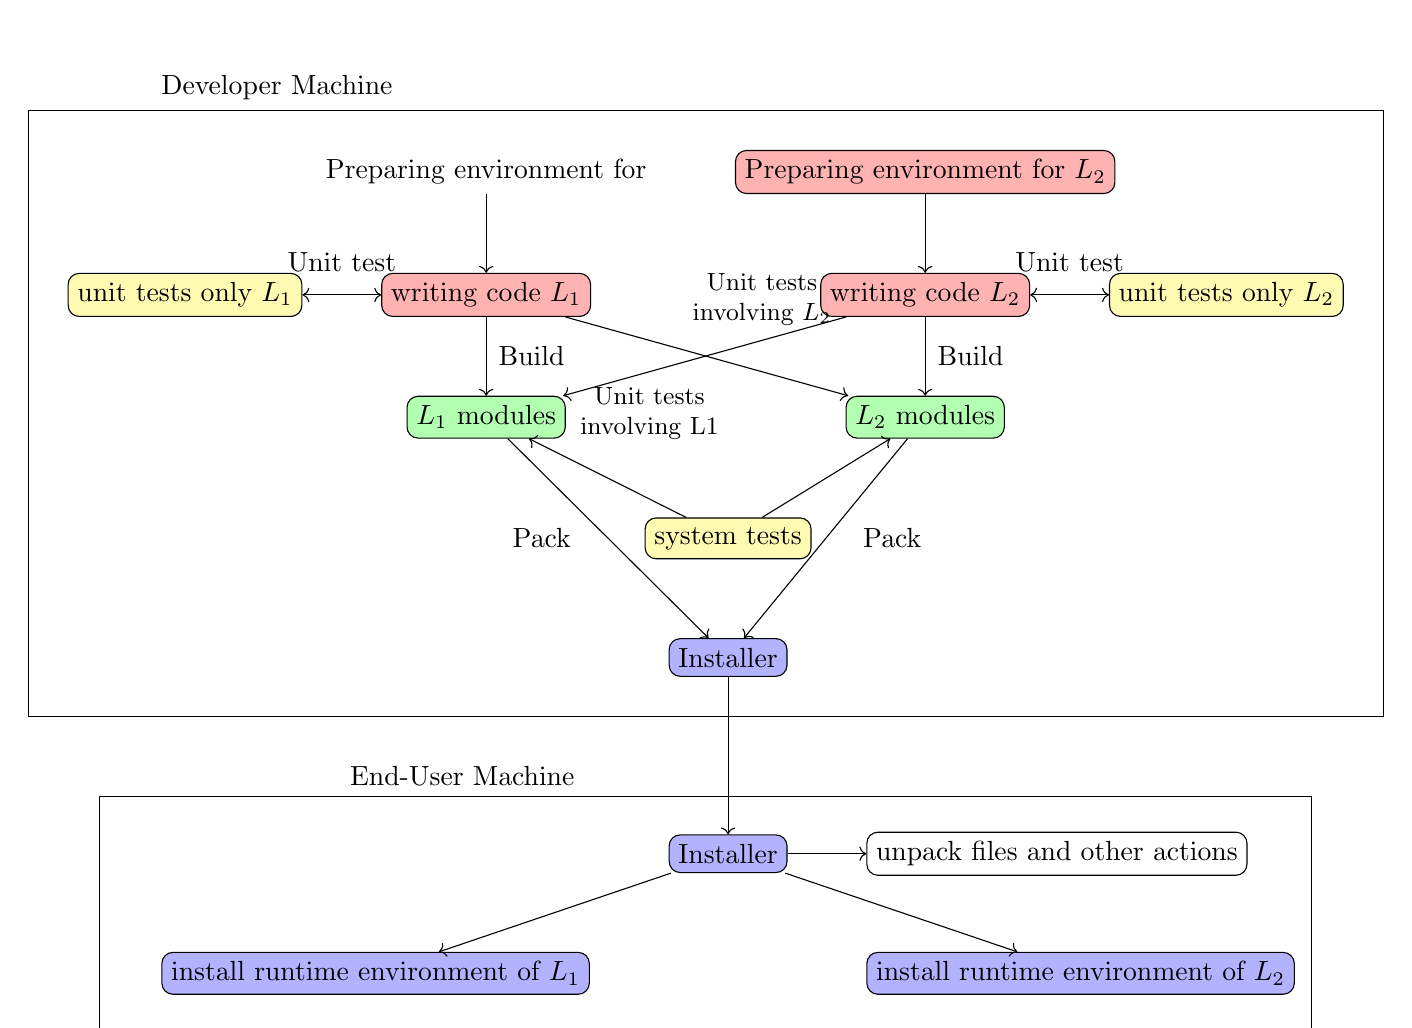
\begin{tikzpicture}[
    dev/.style={rectangle, draw, rounded corners, fill=red!30},
    test/.style={rectangle, draw, rounded corners, fill=yellow!30},
    mod/.style={rectangle, draw, rounded corners, fill=green!30},
    install/.style={rectangle, draw, rounded corners, fill=blue!30},
    dashed/.style={rectangle, draw, rounded corners, fill=white!30}
]

% Developer machine package
\node (Environment1) {Preparing environment for };
\node[dev, right=of Environment1] (Environment2) {Preparing environment for $L_2$};



\node[dev, below=of Environment1] (IDE1) {writing code $L_1$};
\node[dev, below=of Environment2] (IDE2) {writing code $L_2$};

\node[test, left=of IDE1] (TEST1) {unit tests only $L_1$};
\node[test, right=of IDE2] (TEST2) {unit tests only $L_2$};

\node[mod, below=of IDE1] (M1) {$L_1$ modules};
\node[mod, below=of IDE2] (M2) {$L_2$ modules};

\node[test, below right=of M1, xshift=0cm] (SYSTESTS) {system tests};
\node[install, below=of SYSTESTS] (InstallerDev) {Installer};
\begin{pgfonlayer}{background}
\node[fit=(Environment1)(Environment2)(IDE1)(IDE2)(TEST1)(TEST2)(M1)(M2)(SYSTESTS)(InstallerDev), draw, thin, inner sep=0.5cm, label=above left:Developer Machine] (DevMachine) {};
\end{pgfonlayer}

% End-user machine package
\node[install, below=of InstallerDev, yshift=-1cm] (Installer) {Installer};
\node[install, below left =of Installer] (RuntimeInstall1) {install runtime environment of $L_1$};
\node[install, below right=of Installer] (RuntimeInstall2) {install runtime environment of $L_2$};
\node[dashed, right=of Installer] (Unpack) {unpack files and other actions};
\begin{pgfonlayer}{background}
\node[fit=(Installer)(RuntimeInstall1)(RuntimeInstall2)(Unpack), below=of DevMachine, draw, thin, inner sep=0.5cm, label=above left:End-User Machine] {};
\end{pgfonlayer}

Connections

\draw[->] (Environment1) -- (IDE1);
\draw[->] (Environment2) -- (IDE2);
\draw[<->] (IDE1) -- (TEST1) node[midway, above=5pt] {Unit test};
\draw[<->] (IDE2) -- (TEST2) node[midway, above=5pt] {Unit test};
\draw[->] (IDE1) -- (M1) node[midway, right=1pt] {Build};
\draw[->] (IDE2) -- (M2) node[midway, right=1pt] {Build};
\draw[->] (IDE1) -- (M2) node[midway, above=6pt, font=\small, xshift=7mm] {\begin{tabular}{c}Unit tests\\involving $L_2$\end{tabular}};
\draw[->] (IDE2) -- (M1) node[midway, below=6pt, align=left, font=\small, xshift=-7mm] {\begin{tabular}{c}Unit tests\\involving L1\end{tabular}};
\draw[->] (SYSTESTS) -- (M1)  node {};
\draw[->] (SYSTESTS) -- (M2)  node {};
\draw[->] (M1) -- (InstallerDev) node[midway, left=10pt] {Pack};
\draw[->] (M2) -- (InstallerDev) node[midway, right=10pt] {Pack};
\draw[->] (InstallerDev) -- (Installer);
\draw[->] (Installer) -- (RuntimeInstall1);
\draw[->] (Installer) -- (RuntimeInstall2);
\draw[->] (Installer) -- (Unpack);

\end{tikzpicture}
\caption{Multi-PL development process}
\label{fig:process_of_interoperability}
\end{figure}

During this section, without loss of generality (WLOG) assume that $L_1$ is the language in which the developer is writing code, and the usage of $L_2$ can be in two scenarios:
\begin{enumerate}
    \item Write the code in $L_2$ which is used by $L_1$. $L_2$ can also use the code written in $L_1$
    \item No code is written in $L_2$. $L_1$ uses \textit{runnable} modules of $L_2$. Runnable module is a module that can be executed, either by $L_2$ runtime, or directly by the CPU in case of binary.
    \end{enumerate}

The only assumption is that there is an interoperability tool that allows $L_1$ to use $L_2$. For the cases where $L_2$ uses $L_1$, we assume that there is an interoperability tool that allows $L_2$ to use $L_1$.  

\textit{Prepare Environment}: For a developer to develop using $L_1$ and $L_2$, their corresponding runtimes and development tools must be installed on the development machine (e.g., gcc \cite{gcc}, JVM \cite{jvm_specs}, CPython \cite{cpython}) and, if applicable, prepare the environment. For example, \texttt{JAVA\_HOME} which specifies the installation location of JVM, creating symbolic links in \texttt{/usr/bin} in Linux or\texttt{PATH} environment variable on Windows to find the development tools, and many more in non-default scenarios. It does not matter if $L_2$ is embedded within $L_1$ source code (like in CGo \cite{cgo_export_c}) or is written in a different file. Both languages need to be built/executed with some tool. In the case where only $L_2$ runnable modules are used, usually development tools are not necessary.

An interoperability system might have its own environmental requirements. The interoperability system should be clear on its requirement in the development environment, or create it automatically using an installer script.

\textit{Writing Code}: The developer can write code $L_1$ and $L_2$. Either $L_2$ is embedded within the $L_1$ source code or by its own. This step is not relevant for the use of $L_2$ runnable modules.

\textit{Unit test}: Any code that \textbf{is not dependent} on the other language can be unit tested with the language unit test tools, without additional dependencies required by interoperability, as shown by the \emph{Unit test} arrows in figure \ref{fig:process_of_interoperability}.

Any code that \textbf{is dependent} on the other language cannot be tested without building the other language dependencies first. Note that the case of "code embedding", where $L_2$ source code is embedded within $L_1$ source code, makes no difference as the dependencies of a unit test need to be built before it can execute. This is shown by \emph{Unit tests involving $L_1$} and \emph{Unit tests involving $L_2$} arrows. In the case of using runnable modules of $L_2$, there are no unit tests for $L_2$, but $L_1$ unit tests can use runnable modules of $L_2$.

The interoperability system must mitigate the use of the system during unit tests. There should be no constraints imposed by the interoperability system that change behavior or prevent the usage of a unit test tools.

\textit{Build}: The building of the source codes is done using the development tools of the corresponding language. In some cases, the building tools of $L_2$ might be embedded or used by the building tools of $L_1$, but, nevertheless, the source code of $L_2$ must be built either way. For some PLs (e.g., Python \cite{cpython}, CLing C++ interpreter \cite{Cling}), there is no build step, and their runtime interprets the source code directly. For these languages, this step is not applicable. Also, in the case where the developer uses runnable modules of $L_2$, the build step is not required, \textbf{but} the runnable modules might be used by $L_1$ as they are a dependency of some of the $L_1$ code.

It is important to point out, that the \textit{build} step can become complex in the scenario of writing both in $L_1$ and $L_2$, as building the dependencies might require multiple usage of $L_1$ and $L_2$ building tools, based on the dependency tree. The complexity of this step is also discussed in \cite{multilingual_systems_constructed}. Build-oriented languages such as CMake \cite{cmake} or frameworks such as SCons \cite{scons} can help, but it may remain a complex topic that should be addressed. We will not dwell on this further to avoid straying away from the main focus of the article.

The interoperability system can be part of the build process. For example, adding glue code to bind the programming languages (e.g., SWIG \cite{swig}). The system should not \emph{replace} the existing building tools, as this could end up as a language port or as another compiler.

\textit{System Tests}: The system tests are tests running on the entire built application or system. These require all the runnable modules of the application available. In this step, the interoperability system is used by the runnable modules.

\textit{Pack}: In applications that require packing into an installer, usually applications that run on an end-user machine, besides packing all the files and scripts, the generated installer should add the dependencies for $L_1$ and $L_2$ runtimes and their environmental requirements (e.g., environment variables).

The interoperability system might have its own requirements and dependencies in the end-user machine. The system should be clear about the requirements, dependencies, and environmental requirements so the developers can incorporate them within their own installer, or validate them on the deployed machine.

Once we illustrated a typical multi-PL development cycle, we can continue to discuss the system itself and check if there are issues or challenges in either of the steps.


\section{Using an entity in runnnable code} \label{sec:using_foreign_entity}

It is important to break down the anatomy of using an entity in a different runtime. Assume $L_1$ and $L_2$ are programming languages and there is a mechanism that allows us to make a call from $L_1$ to $L_2$. Note that we cannot assume that they are executed on the same runtime. $L_1$ could be binary while $L_2$ runs on the virtual machine of the.NET framework \cite{ms_dotnet}, or $L_2$ might compile to binary but bring the whole framework like Go \cite{golang}.

First, in figure \ref{fig:calling_c} we break down the use from C to another C function (execute) or global (read/write) which resides in a different dynamic library, which is not loaded into the OS process, therefore the link/bind is done at runtime. We will generalize this to an arbitrary programming language, runtime and runnable module. Note that conceptually, a \textit{similar} process happens for any function in different modules by the compiler at compile time.

\begin{figure}[h]
\centering
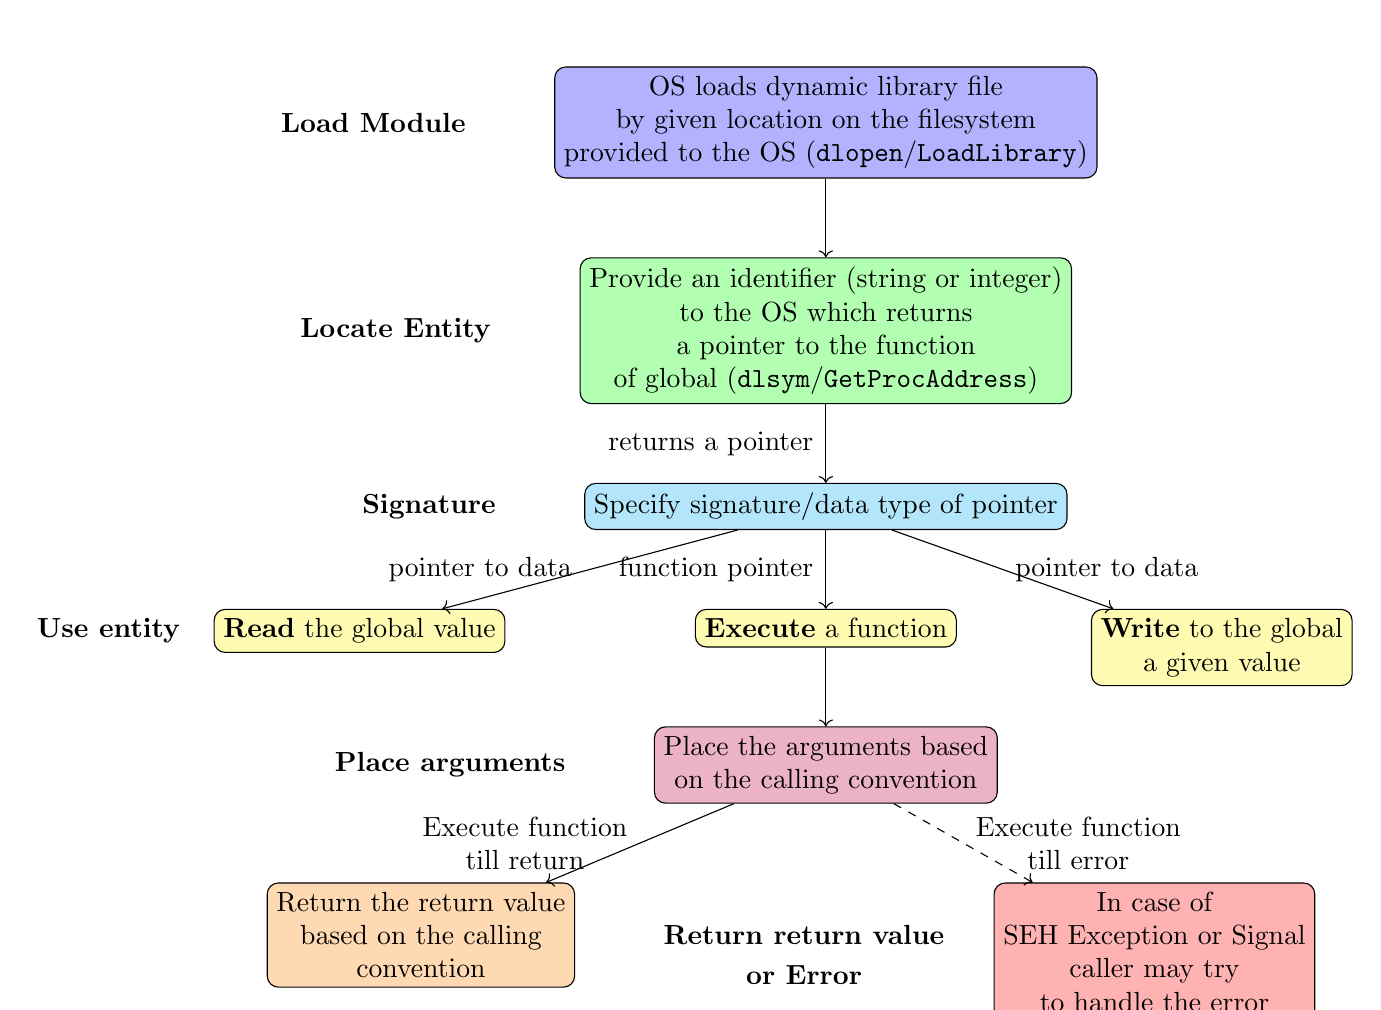
\begin{tikzpicture}[
        loadmodule/.style={rectangle, draw, rounded corners, fill=blue!30},
        locate/.style={rectangle, draw, rounded corners, fill=green!30},
        sig/.style={rectangle, draw, rounded corners, fill=cyan!30},
        useentity/.style={rectangle, draw, rounded corners, fill=yellow!30},
        args/.style={rectangle, draw, rounded corners, fill=purple!30},
        rets/.style={rectangle, draw, rounded corners, fill=orange!30},
        err/.style={rectangle, draw, rounded corners, fill=red!30},
    ]

\node[loadmodule, align=center] (LoadModule) {OS loads dynamic library file\\by given location on the filesystem\\provided to the OS (\texttt{dlopen}/\texttt{LoadLibrary})};
\node [left=of LoadModule] {\textbf{Load Module}};

\node[locate, align=center, below=of LoadModule] (LocateFunctionOrGlobal) {Provide an identifier (string or integer)\\to the OS which returns\\a pointer to the function\\of global (\texttt{dlsym}/\texttt{GetProcAddress})};
\node [left=of LocateFunctionOrGlobal] {\textbf{Locate Entity}};
\draw[->] (LoadModule) -- (LocateFunctionOrGlobal);

\node[sig, align=center, below=of LocateFunctionOrGlobal] (Sig) {Specify signature/data type of pointer};
\node[left=of Sig] {\textbf{Signature}};
\draw[->] (LocateFunctionOrGlobal) -- (Sig) node [midway, left=1pt, align=center] {returns a pointer};

\node[useentity, align=center, below=of Sig] (UseFunction) {\textbf{Execute} a function};
\node[useentity, align=center, below left=of Sig] (UseGetGlobal) {\textbf{Read} the global value};
\node[useentity, align=center, below right=of Sig, xshift=-20] (UseSetGlobal) {\textbf{Write} to the global\\a given value};
\node [left=of UseGetGlobal, xshift=20] {\textbf{Use entity}};
\draw[->] (Sig) -- (UseFunction) node[midway, left=1pt, align=center] {function pointer};
\draw[->] (Sig) -- (UseGetGlobal) node[midway, left=3pt, align=center] {pointer to data};
\draw[->] (Sig) -- (UseSetGlobal) node[midway, right=1pt, align=center] {pointer to data};

\node[args, align=center, below=of UseFunction] (Args) {Place the arguments based\\on the calling convention};
\node [left=of Args] {\textbf{Place arguments}};
\draw[->] (UseFunction) -- (Args);

\node[rets, align=center, below left=of Args] (Rets) {Return the return value\\ based on the calling\\convention};
\draw[->] (Args) -- (Rets) node [midway, left=1pt, align=center] {Execute function\\till return};
\node [right=of Rets] (RetText) {\textbf{Return return value}};
\node [below=of RetText, yshift=28] {\textbf{or Error}};

\node[err, align=center, below right=of Args, xshift=-30] (Error) {In case of\\SEH Exception or Signal\\caller may try\\to handle the error};
\draw[->, dashed] (Args) -- (Error) node [midway, right=1pt, align=center] {Execute function\\till error};
\end{tikzpicture}

\caption{Loading and using a function or global in C}
\label{fig:calling_c}
\end{figure}

Figure \ref{fig:calling_c} illustrates the following steps:
\begin{enumerate}
    \vspace{-2mm}\item Load Module - loads the dynamic library using the OS API by providing the path of the module on the filesystem.
    \vspace{-2mm}\item Locate Entity - the program needs to locate the entity it needs from within loaded module. By providing an identifier, the OS locates the entity and returns a {handle}. In C, the handle is a pointer to an unknown underlying type - \texttt{void*}.
    \vspace{-2mm}\item Signature - The program need to explicitly state the type of the handle. In C, the program must cast the \texttt{void*} to the correct type. In case of a function, the program needs to explicitly state (by casting) the signature of the type.
    \vspace{-2mm}\item Use entity - The program can now use the entity. Either read, write, or execute. In the case of C, read from memory, write to memory, or execute a function.
    \vspace{-2mm}\item In the case of execution:
    \begin{enumerate}
        \vspace{-2mm}\item Place arguments - Place the arguments in their expected location and form for the call. In case of C, arguments layout depends on the calling convention.
        \vspace{-2mm}\item Return values - Placed in the location and form for the caller to read them after execution. In case of C, only one return value is supported, and its location and form depends by the the calling convention.
        \vspace{-2mm}\item Error - In case of an error. Either the error returns as a return value or interrupts/exceptions, which are a common method in operating systems (SEH Exception \cite{seh_exception} in Windows or signals in Linux \cite{unix_signal}) and programming languages. In the case of an C, error usually returns in return value, or OS errors which raise SEH exceptions or signals which the code can handle and try to recover.
    \end{enumerate}    
\end{enumerate}


Unlike using a C entity from C, when generalizing to arbitrary $L_1$ and $L_2$, there are assumptions that we can make in C to C scenario, but not in $L_1$ to $L_2$. For the rest of the section, we assume $M$ is a mechanism that allows $L_1$ to use or communicate with $L_2$.

We assume that C can load C-compliant runnable module, i.e. dynamic library module, but this is not true for any runnable module or model. In the case of loading an arbitrary runnable module, $L_1$ would need to load a runtime that can execute the runnable module before actually loading it. For example, assume $L_1=$Python $L_2=$Java and the module is JAR, the runnable module of Java Virtual Machine. Python needs to first load the JVM before it can load the JAR. As specified before, we currently assume that $M$ allows Python to load the JVM. This is required in any in-process approach, that is, use $L_2$ in the same OS-process of $L_1$.

There are two models to use $L_2$ outside of $L_1$ OS process: 
\begin{enumerate*}
\item shared memory using memory mapping
\item message passing through communication technology 
\end{enumerate*}.

In shared memory model, $M$ is executing and/or sharing memory with an OS process running the $L_2$ runtime and providing an API for $L_1$ to load a runnable module and/or entity of $L_2$. In message passing model, $M$ is executing and/or connecting with an OS process running $L_2$ runtime and provide an API that allows $L_1$ to load runnable module and/or entity of $L_2$. 

In all models described above, $L_1$ first needs to load something of $M$ (at runtime or link at compile time) to load the $L_2$ runtime, or share memory with another process or communicate with another process that runs $L_2$ runtime.

Therefore, in both models, for $L_1$ to use an entity in $L_2$, $L_1$ needs to \textbf{load a dependency}, which is part of $M$ or using $M$, into the $L_1$ OS process, before it can use the $L_2$ runnable module and an entity.

Note that all the interoperability mechanisms described in \cite{empirical_multi_lingual} \cite{toward_description_of_interop} \cite{polyfax}, fall into one of the models described above.

Once the dependency of $M$ is loaded, $L_1$ can use $M$ to load a runnable module. Notice, that in some cases $L_2$ might not require specifying a module as the required entity is global in the runtime (for example, \texttt{dict} in Python), in this case loading the module step can be skipped.

Another key point in figure \ref{fig:calling_c} that cannot be generalized to arbitrary $L_1$ and $L_2$ is the read and write operations. Although C can directly access the memory of the returned pointer to read or write, we cannot assume that $L_1$ can access the memory of $L_2$. However, we can assume that $M$ can \textbf{execute} code that reads the data from $L_2$ and returns it to $L_1$, or write the data given from $L_1$ to $L_2$ runtime. Therefore, in the general case, we replace \textit{Read} operation with \textit{Execute} operation of a function that returns data from $L_2$ runtime and name it a \textit{getter}. Similarly, we do the same for the \textit{Write} operation and replace it with the \textit{Execute} operation of a function that writes to $L_2$ runtime and name it a \textit{setter}.

It is important to note that even in the general case, the signature of the entity is critical, as the program needs to know how to address the data it receives of returns, regardless if it is passed by shared memory or in a string-encoded message. The data types and structure of the underlying memory or message are the signature.

The last key point that we need to clarify is that $L_2$ might support incompatible return values and arguments count, size, or anything else compared to $L_1$. For now, we assume that $M$, as a mechanism for interoperability between $L_1$ and $L_2$, addresses this issue.

\begin{figure}[h]
\centering
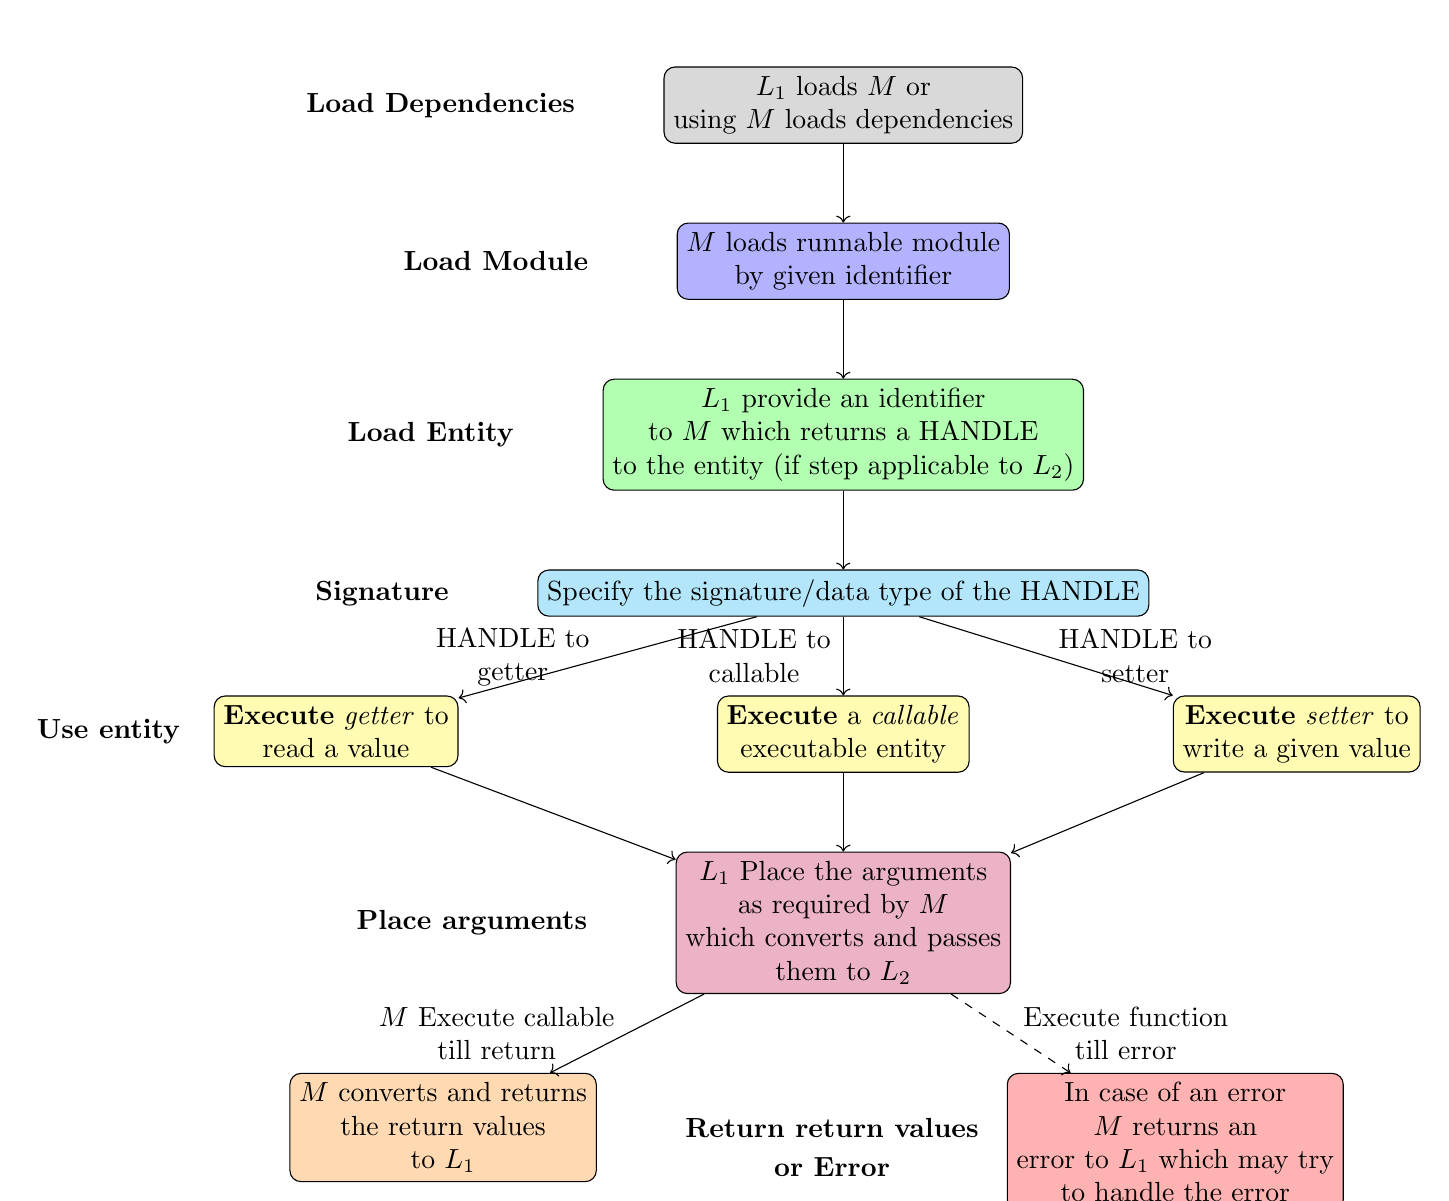
\begin{tikzpicture}[
    loaddeps/.style={rectangle, draw, rounded corners, fill=gray!30},
    loadmodule/.style={rectangle, draw, rounded corners, fill=blue!30},
    locate/.style={rectangle, draw, rounded corners, fill=green!30},
    sig/.style={rectangle, draw, rounded corners, fill=cyan!30},
    useentity/.style={rectangle, draw, rounded corners, fill=yellow!30},
    args/.style={rectangle, draw, rounded corners, fill=purple!30},
    rets/.style={rectangle, draw, rounded corners, fill=orange!30},
    err/.style={rectangle, draw, rounded corners, fill=red!30}
 ]

\node[loaddeps, align=center] (LoadDeps) {$L_1$ loads $M$ or\\using $M$ loads dependencies};
\node [left=of LoadDeps] {\textbf{Load Dependencies}};

\node[loadmodule, align=center, below=of LoadDeps] (LoadEntityModule) {$M$ loads runnable module\\by given identifier};
\draw[->] (LoadDeps) -- (LoadEntityModule);
\node [left=of LoadEntityModule] {\textbf{Load Module}};

\node[locate, align=center, below=of LoadEntityModule] (LocateEntity) {$L_1$ provide an identifier\\to $M$ which returns a HANDLE\\to the entity (if step applicable to $L_2$)};
\draw[->] (LoadEntityModule) -- (LocateEntity);
\node [left=of LocateEntity] {\textbf{Load Entity}};

\node[sig, align=center, below=of LocateEntity] (Sig) {Specify the signature/data type of the HANDLE};
\draw[->] (LocateEntity) -- (Sig);
\node [left=of Sig] {\textbf{Signature}};

\node[useentity, align=center, below=of Sig] (UseFunction) {\textbf{Execute} a \textit{callable}\\executable entity};
\node[useentity, align=center, below left=of Sig] (UseGetter) {\textbf{Execute} \textit{getter} to\\ read a value};
\node[useentity, align=center, below right=of Sig, xshift=-20] (UseSetter) {\textbf{Execute} \textit{setter} to\\write a given value};
\node [left=of UseGetter, xshift=20] {\textbf{Use entity}};
\draw[->] (Sig) -- (UseFunction) node[midway, left=1pt, align=center] {HANDLE to\\callable};
\draw[->] (Sig) -- (UseGetter) node[midway, left=3pt, align=center] {HANDLE to\\getter};
\draw[->] (Sig) -- (UseSetter) node[midway, right=1pt, align=center] {HANDLE to\\setter};

\node[args, align=center, below=of UseFunction] (Args) {$L_1$ Place the arguments\\as required by $M$\\which converts and passes\\them to $L_2$};
\node [left=of Args] {\textbf{Place arguments}};
\draw[->] (UseFunction) -- (Args);
\draw[->] (UseGetter) -- (Args);
\draw[->] (UseSetter) -- (Args);

\node[rets, align=center, below left=of Args] (Rets) {$M$ converts and returns\\the return values\\to $L_1$};
\draw[->] (Args) -- (Rets) node [midway, left=1pt, align=center] {$M$ Execute callable\\till return};
\node [right=of Rets] (RetText) {\textbf{Return return values}};
\node [below=of RetText, yshift=28] {\textbf{or Error}};

\node[err, align=center, below right=of Args, xshift=-30] (Error) {In case of an error\\$M$ returns an\\error to $L_1$ which may try\\to handle the error};
\draw[->, dashed] (Args) -- (Error) node [midway, right=1pt, align=center] {Execute function\\till error};

\end{tikzpicture}
\caption{Calling an $L_2$ entity from $L_1$ runtime}
\label{fig:calling_fentity}
\end{figure}

Figure \ref{fig:calling_fentity} breaks down the use of an entity in $L_2$ runtime from $L_1$ runtime, and it presents the mains stages $M$ performs to use an entity:
\begin{enumerate*}
\item Load dependencies
\item Load module (skipped if not applicable to $L_2$)
\item Load entity
\item Specify entity signature
\item Use the entity
\item Place arguments
\item Return return values or error
\end{enumerate*}

An interoperability system needs to provide an abstraction layer to any given $M$, while imposing the least constraints over $M$, providing the developer the ability to perform the main steps, as presented above, in a uniform way.

The operating system provides application the ability to load and run binaries in the their chosen executable format, for example, PE (Portable Executable \cite{portable_executable} in Windows, or ELF (Executable and Linkable Format) in its different forms in Linux, MacOS and such. The interoperability system should act as an extension of the operating system to extend the ability to load and execute code that is not runnable just by the CPU, but by an arbitrary runtime using interoperability mechanisms as shown in figure \ref{fig:interoperability_system_layer}, where each pair of mechanisms that supports $L_i$ must not be aware of the mechanisms of $L_j$. The reason why two mechanisms are required (which in some cases could be the same mechanism) is to provide a full-duplex interaction. The interoperability system should also support a half-duplex interaction for flexibility to allow cases where a mechanism is not implemented or not available.

\begin{figure}[h]
\centering
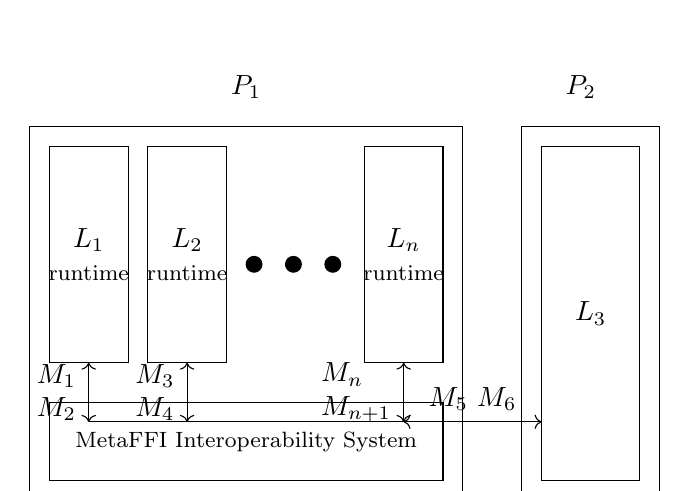
\begin{tikzpicture}

  % Main rectangles
  \draw (1.5,15.25) rectangle (7,10.5);
  \draw (1.75,11.75) rectangle node {\smaller{MetaFFI Interoperability System}} (6.75,10.75);
  \draw (1.75,15) rectangle node [align=center] {$L_1$\\\smaller{runtime}} (2.75,12.25);
  \draw (3,15) rectangle node [align=center] {$L_2$\\\smaller{runtime}} (4,12.25);
  \draw (5.75,15) rectangle node [align=center] {$L_n$\\\smaller{runtime}} (6.75,12.25);

  % Circles
  \draw [fill={rgb,255:red,0; green,0; blue,0}] (4.35,13.5) circle (0.1cm);
  \draw [fill={rgb,255:red,0; green,0; blue,0}] (4.85,13.5) circle (0.1cm);
  \draw [fill={rgb,255:red,0; green,0; blue,0}] (5.35,13.5) circle (0.1cm);

  % Arrows
  \draw [<->] (2.25,11.5) -- (2.25,12.25) node [midway, left=1pt, align=left] {$M_1$\\$M_2$};
  \draw [<->] (3.5,11.5) -- (3.5,12.25) node [midway, left=1pt, align=left] {$M_3$\\$M_4$};
  \draw [<->] (6.25,11.5) -- (6.25,12.25) node [midway, left=1pt, align=left] {$M_n$\\$M_{n+1}$};
  \draw [-] (2.25,11.5) -- (6.25,11.5);

  % Second section
  \draw (7.75,15.25) rectangle (9.5,10.5);
  \draw (8,15) rectangle node [align=center] {\normalsize $L_3$} (9.25,10.75);
  \draw [<->] (6.25,11.5) -- (8,11.5) node [midway, above=0.5pt, align=left] { $M_5$   
  $M_6$};

  % Nodes
  \node [] at (4.25,15.75) {$P_1$};
  \node [] at (8.5,15.75) {$P_2$};

\end{tikzpicture}
\caption{Interoperability System Layer}
\label{fig:interoperability_system_layer}
\end{figure}

In the following sections, we will systematically explore the stages involved in using an entity as explained so far. We will begin by discussing each stage in detail, examining previous work in the field to highlight the evolution and context of our approach. Furthermore, we will elucidate our design decisions, emphasizing how they enhance interoperability and address existing challenges, thereby demonstrating the innovation and efficiency of the MetaFFI system.

We also define $M_1$ as an interoperability mechanism that allows $L_1$ to interact with the interoperability system and $M_2$ allows the interoperability system to interact with $L_2$. We currently mainly focus on $M_2$, as $L_1$ can use $M_1$ to interacts with the interoperability system. We will address $M_1$ in section~\ref{sec:pl_api}.

\subsection{Pluggable Design} \label{sec:pluggable_design}
As shown in figure \ref{fig:interoperability_system_layer}, for a runtime of a PL to communicate with the interoperability system, it requires a pair of interoperability mechanisms for full-duplex, or at least one for half-duplex interoperability.

We define an interoperability system plugin as a module that encapsulates a pair (or single for half-duplex) of mechanisms for a specific PL runtime (figure \ref{fig:interoperability_system_layer_with_plugins}). Note that a plugin is not dependent on any other plugins, therefore the effort required to implement a plugin to support a PL runtime is independent. This means that using an interoperability system, to provide interoperability between $N$ programming language, the system requires $N$ plugins ($2n$ mechanisms), that is in contrast of direct interoperability between all $N$ PLs, which requires $n^2$ mechanisms.

\begin{figure}[!h]
\centering
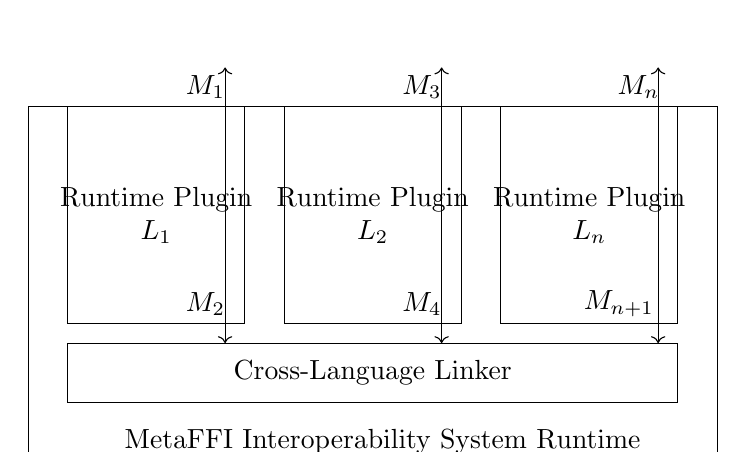
\begin{tikzpicture}
 \draw  (5,9) rectangle (13.75,4.5);
 \draw  (5.5,9) rectangle  node [align=center] {Runtime Plugin\\$L_1$} (7.75,6.25);
 \draw  (8.25,9) rectangle  node [align=center] {Runtime Plugin\\$L_2$} (10.5,6.25);
 \draw  (11,9) rectangle  node [align=center] {Runtime Plugin\\$L_n$} (13.25,6.25);
 \draw [<->] (7.5,9.5) -- (7.5,6);
 \draw [<->] (10.25,9.5) -- (10.25,6);
 \draw [<->] (13,9.5) -- (13,6);
 \draw  (5.5,6) rectangle  node {Cross-Language Linker} (13.25,5.25);
 \node [font=\normalsize] at (9.5,4.75) {MetaFFI Interoperability System Runtime};
 \node [font=\normalsize] at (7.25,9.25) {$M_1$};
 \node [font=\normalsize] at (7.25,6.5) {$M_2$};
 \node [font=\normalsize] at (10,9.25) {$M_3$};
 \node [font=\normalsize] at (10,6.5) {$M_4$};
 \node [font=\normalsize] at (12.5,6.5) {$M_{n+1}$};
 \node [font=\normalsize] at (12.75,9.25) {$M_n$};
\end{tikzpicture}
\caption{Interoperability System Layer Plugins}
\label{fig:interoperability_system_layer_with_plugins}
\end{figure}

As the interoperability plugin encapsulates interoperability mechanisms, the plugin needs provide an API to use the mechanisms in a unified manner. This is done by implementing an interface defined by the MetaFFI interoperability system that reflects the stages shown in figure \ref{fig:interoperability_system_layer}.

MetaFFI supports four types of components that extends the system:
\begin{itemize}
    \item Runtime plugin
    \item Compiler plugin
    \item IDL plugin
    \item PL API
\end{itemize}

In most cases, only the runtime plugin is mandatory, where the others are to provide additional features that make MetaFFI even simpler to use, as discussed in sections \ref{sec:pl_api} and \ref{sec:using_entity_in_source_code} and indicated in section \ref{sec:survey}. In the following sections we discuss mainly the runtime plugin.

Note that the concept of a runtime is extended beyond just a programming language runtime, but a runtime includes any interoperability operation of read, write, and execute. For example, an interoperability plugin for Windows implements interoperability with shared objects (\texttt{.so} files) in Linux using Windows Subsystem for Linux (WSL \cite{wsl}), or a plugin that implements the REST protocol efficiently and makes it available to all other available programming languages without any additional effort, or a plugin for SQLite that provides functions that calls stored procedure.

\subsection{Loading Dependencies} \label{sec:loading_dependencies}
The first stage is \textit{Loading Dependencies}, as explained in \ref{sec:using_foreign_entity}.

There are two ways $M_2$ can be loaded, explicitly or implicitly. Explicit loading occurs when the code that uses $M_2$ calls functions to load the runtime or dependencies. For example, the Java Native Interface (JNI \cite{jni}) provides the function \texttt{JNI\_CreateJavaVM} to load the JVM. Another example, to use the Microsoft Component Object Model (COM \cite{com_component}) component, either for the in-process or out-of-process interoperability, the user of COM needs to initialize using \texttt{CoInitializeEx}. Using explicit initialization, the user of $M_2$ can configure the loaded dependencies.

In implicit loading, the initialization is not called explicitly, but as a side-effect. For example, Go \cite{golang}, a programming language compiles to binary, allows its developers to build a C-compatible dynamic library where the Go runtime is loaded implicitly when the OS process loads the dynamic library.  Another example is again the COM component using C\# \cite{c_sharp}, a programming language that runs on the Microsoft.NET virtual machine, where the .NET can be configured to load the COM component without explicit code by the developer. With that, for none default configuration, .NET allows also explicit initialization. There are more examples like Python C-extension \cite{pyhton_c_extension} and RUST \cite{rust} programming language.

The interoperability system that uses $M_2$, needs to provide the user the ability to pass arguments for the explicit loading/initialization process of $M_2$, or not pass anything in the case of implicit initialization. This is the \texttt{\textbf{LoadRuntime(configurations and settings)}} entry in the MetaFFI API provided to the user of the system.

It is worth mentioning that implicit loading might also accept arguments by out-of-band means like environment variables, configuration files, and such. In MetaFFI, we focus on passing arguments explicitly through the programming language, as a program language interoperability system. In our view, the implicit configuration done by the environment is handled by other mechanisms such as Linux containers \cite{container} and Python virtual environments \cite{python_virtual_environment}.

\subsection{Load Module}

This stage allows the user of the interoperability system to tell $M_2$ where the runnable code of the entity is located. Although $M$ must know where the code resides, this step may be optional.

The syntax of the location of a runnable module or code varies between runtimes. Some examples are file on the filesystem (C, C++), URLs (JavaScript), package names (Python), and not specifying any location at as the runnable modules or their locations predefined or built-in.

The interoperability system that uses $M_2$, needs to provide the user with the ability to pass arguments on the location of the runnable module containing the entity, or not pass anything in the case it is not required. This argument is the first of the \texttt{\textbf{LoadEntity(Module Location, ...)}} entry in the MetaFFI API provided to the system user. It is combined as both actions are part of locating the entity, and we wish to reduce the amount of code required to use the system.

\subsection{Load Entity}

In order to load the entity, $M_2$ requires one or more identifications to locate the entity. For example, COM would require and integer which signifies the location of the entity in a function table. C needs an exported function name (or integer in Windows) to locate the function. REST requires a URL containing the path to the function.

Moreover, also metadata about the entity might also be required, for example, JNI behaves differently if it needs to load a method, static method, field, or static field.

In order to support a variety of inputs, the interoperability system that uses $M_2$, accepts a map of identifications, which internally maps the given arguments to $M_2$. We can combine the argument \textit{Module Location} into the map. The module location entry would be filled in the cases required. The entry \textit{LoadEntity} is changed to \texttt{\textbf{LoadEntity(Entity Path, ...}} in the MetaFFI API, where the entity path is the map described above.

\subsection{Signature}

For MetaFFI to execute $M_2$ to perform read/write/execute operations, it needs to know the underlying data type of the entity.

Defining the signature is made out of two challenges:
\begin{itemize}
    \item How to define an entity signature for arbitrary PL?
    \item How to define the data types for arbitrary PL?
\end{itemize}

\subsubsection{Entity Signature}
A common usage to define an entity for arbitrary PL is to use an interface definition language (IDL \cite{idl_wikipedia}). IDL is text that contains the definition (i.e., signature) of a single entity or multiple entities. The developer writes the IDL, which $M_2$ uses to detect the signature of (sometimes also to locate) the entity. Some IDLs format is built to "feel" like a pseudo-programming language syntax for easier usage, like COM and SWIG (reminds of C) and Google Protocol Buffers (protobuf \cite{protobuf_dev_guide}) and Thirft (reminds of Java/C\#). Other IDLs use well-known text-based formats like OpenAPI/Swagger \cite{openapi} using JavaScript Object Notation (JSON \cite{json_rfc}) or YAML Ain't Markup Language (YAML \cite{yaml_rfc}) formats, or Microsoft SOAP (\cite{soap_rfc}) using eXtensible Markup Language (XML \cite{xml_rfc}). In summary, the IDL is a document authored manually that serves to explicitly define the signature of entities. A compiler compiles the IDL into the code that performs the interoperability. It is important to note that as the IDL is at compile time, the generated code can be optimized to the specific function.

Although IDL usage is common in interoperability mechanisms, its usage imposes a significant overhead \cite{empirical_multi_lingual} \cite{polispin}, especially when using large $3^{rd}$ libraries. To overcome the overhead, tools were created to generate IDLs automatically by parsing the source code.

LibFFI \cite{libffi} is a well-known interoperability library to load and use C exported entities. LibFFI does not use an IDL text, instead, the developer defines the signature using LibFFI API, which is evaluated during runtime.

CTypes \cite{python_ctypes}, an interoperability mechanism from Python to C, uses LibFFI internally and takes a step further to try to guess the signature of the C entity during runtime, unless explicitly defined by the developer using Python code. While this approach can be convenience in some scenarios, it could be frustrating in case the guessed signature is wrong as the outcome is undefined.

In the paper \cite{polyspin}, the authors criticize the usage of IDL and the explicit need of a developer to define the signature of the entity. The authors present Polyspin, a technique to replace IDL usage by using a \textit{Matcher} from $L_1$ to $L_2$. When calling from $L_1$ to $L_2$, the Matcher automatically matches between data types, removing the developer from explicitly defining the signatures. The issue with this approach is that a matcher is from specific $L_1$ to specific $L_2$, which means that for $N$ languages, we would need $N^2$ Matchers.

MetaFFI provides both LibFFI and IDL approaches, but in the case of IDL, it is generated automatically, similarly to IDL generation tools, but keeps the IDL internally to the system. The system users can choose the approach that is more suitable based on their needs, generate $L_1$ code at compile time, or define the signature inside the $L_1$ code. Each approach has its own pros, cons, and personal preferences.

In the \textit{LoadEntity} entry in MetaFFI API provided to the user, the second and third arguments are arrays to specify the signature of the entity: \texttt{\textbf{LoadEntity(Module Location, Arguments data types, Return values data types)}}. This approach is similar to the LibFFI approach in specifying the signature on runtime. As shown in section \ref{sec:using_foreign_entity}, write and read operations are execute operations of \textit{getters} and \textit{setters}, therefore, they also have arguments and return values. For example, a setter of a structure field has two arguments, an instance of the structure and the value to set. A getter of an object field has one argument, an instance of the object, and one return value, the value of the field.

MetaFFI also provides an automatic generation of the IDL from the source code and a compiler that generates the interoperability code, using the runtime technique, as explained in the previous paragraph, from the IDL. For that reason, this feature is optional, but useful for interoperating with large libraries. Although MetaFFI IDL is not meant to be human-readable, it is based on a text-based JSON format. It is important to note that MetaFFI IDL created from one PL can generate source code for all other PLs.

Many of the interoperability mechanisms are built so that the data can always be copied from one PL to another. For that reason, all data types must be completely defined down to their primitives. In MetaFFI, instead of always copying the data, a PL can hold a reference, called a handle, to an entity in a different runtime. The system does not necessarily need to know anything about what is behind the handle, besides the specific operations the user wants to use on that entity. Due to that, we are able to mitigate challenges that other IDL systems cannot handle.
 
For example, some challenges MetaFFI handles are key-value and named arguments. We do not state in the IDL these specific features in the IDL but allow the flexibility of PLs to provide metadata about the arguments and return values. For example, the Python function:\\
\texttt{mixed\_params(a, /, b, *, c='default')}\\
In this function, the arguments are:
\begin{itemize}
    \item \texttt{a} is positional, must be the first
    \item \texttt{b} is either positional (second) or named, for example \texttt{b=5} than its position is not relevant
    \item \texttt{c} is only named, and if not specified has a default value
\end{itemize}

For this function, in Python, either of those calls is valid and correct:
\begin{itemize}
    \item \texttt{mixed\_params(1, 2)} - \texttt{c} would get the default value
    \item \texttt{mixed\_params(1, c=3, b=2)} - \texttt{c} is named argument and \texttt{b} can be named, therefore it is correct 
\end{itemize}

By using metadata over the arguments, MetaFFI (and its relevant plugin, which we discuss in section \ref{sec:pluggable_design}) can state that \texttt{b} is positional or named, and \texttt{c} is named. We will discuss later how a PL that does not support these features can make the call such that the interoperability system understands what the developer wants.

Another example is variadic arguments. Another example in also in Python, as it supports two types of variadic arguments is:\\
\texttt{mixed\_vars(*args, **kwargs)}\\
In this function, the arguments are:
\begin{itemize}
    \item \texttt{args} positional variadic arguments - an array or values passed to the function.
    \item \texttt{kwargs} keyword (or named) variadic arguments - a dictionary with key-value pairs, mapping the name of the argument to its actual value
\end{itemize}

For this function, in Python, either of those calls is valid and correct:
\begin{itemize}
    \item \texttt{mixed\_vars(1, 2, c=3,d=4)} - \texttt{args} contains 1 and 2, and \texttt{kwargs} contain \texttt{c=3} and \texttt{d=4} 
    \item \texttt{mixed\_params(1, 2)} - \texttt{args} contains 1 and 2, and \texttt{kwargs} is empty
    \item \texttt{mixed\_params(c=3,d=4)} - \texttt{args} is empty, and \texttt{kwargs} contain \texttt{c=3} and \texttt{d=4}
\end{itemize}

Similarly to the previous example, MetaFFI uses metadata over the arguments to specify \texttt{args} is positional variadic and \texttt{kwargs} is keyword variadic.

It is crucial that the interoperability system is unaware of these PL specific features to maintain the level of abstraction. The system should only provide a way to specify metadata that can be used by PL specific plugins.

\subsubsection{Data Types}
Many interoperability mechanisms that support more than one PL provide an interoperable data-type system. Most type systems provide the common primitives in many PLs, like the different types of integers (8 bit integer, 16 bit integer, etc.), floating points, boolean, null, string and so on.

Some systems also provide types for less common data types. In Microsoft VARIANT \cite{com_variant}, the type system used in COM, there are many primitives in the type system. For instance, currency (\texttt{VT\_CY}), a function (\texttt{VT\_DISPATCH} called dispatch), error (\texttt{VT\_ERROR}), Date (\texttt{VT\_DATE}) and more. The Object Management Group (OMG \cite{omg_idl}) DDS-XTypes \cite{dds-xtypes}, whose type system is formally defined in the Unified Modeling Language (UML \cite{uml}) is similar to VARIANT, and also supports map and set.

Many data type systems allow one to define complex types. For example, in COM and DDS-XTypes the developer can define a structure containing their primitive types defined within the type system or more complex types already defined. In protobuf, a data type system used for serialization of data to messages (i.e., structures), besides defining custom messages, the developers can define new data types which, eventually, can use only the data types already defined by the type system.

Another common data type is a dynamic type. This type can hold any type within the type system. For example, in COM it is VARIANT data type (\texttt{VT\_VARIANT}). In protobuf, it is a custom type called \textit{Any}, which holds a serialized data (i.e., known data type) and the type ID.

Array and maps are also supported by many types systems, such as DDS-XTypes, protobuf, and Facebook Thrift \cite{thrift}, but some systems (e.g. protobuf) are limited in the types of array they support. For example, a ragged array like \texttt{[1, [2,[3,4]], [5], 6]}.

One of the main limitations of the type systems in interoperability mechanisms is that they try to map all the existing primitives. Any extension or complex types of new types, must derive from these basic primitives of the type system. In an interoperability mechanism, it makes sense, but in an interoperability system, it sets a limit on what the system can express. For example, the Go programming language supports complex numbers as a data type. There is no way to express this data type as a primitive if it is not within the type system. The developer can create a workaround by defining a complex type with the required fields, and then convert the fields to create the primitive, but it requires the developer to use $L_2$ instead of just using it. We should point out that COM supports expressing an unknown type using \texttt{VT\_UNKNOWN}. MetaFFI takes a similar approach to COM for using unknown types, although COM assumes that this unknown entity is a COM object (i.e., implements an interface called \texttt{IUNKOWN}), MetaFFI does not make such assumption.

Another limitation is that all complex types must be predefined, recursively, down to its primitives. In this case the developer needs to call a function that accepts a complex type, the developer might invest a lot of effort just to define the type. MetaFFI does not require this, as it does not require complete information about the underlying data type by using another level of indirection. This also has an effect on generating IDLs for PLs using loose types or duct typing (e.g. Python) where the data types are not explicitly defined in the source code. While existing type systems can state that types are dynamic, they actually state that the type is dynamic for the set of types within their type system, which is not necessarily the case (like the complex type example in Go).

\subsection{Use Entity, Place Arguments and Return return values}
As explained above, write and read operations are translated to execute operations, therefore, any write or read is done by execution of a callable in $M$. To execute, $L_1$ passes the arguments to the interoperability system using $M_1$, which in turn, the interoperability system places arguments using $M_2$ which invokes an operation in $L_2$.

Using the entity is constructed of two parts, making the call in $L_1$ and exchanging the arguments and return values.


\subsubsection{Making the call:} When making the call, one way to design the system is such that $L_1$ would call MetaFFI a \textit{cross-call} function in its API, and MetaFFI would redirect the call to $L_2$. This approach is a bit cumbersome and might even incur a performance hit. It would require MetaFFI to redirect the call to the relevant plugin of $L_2$ (from all the other available PLs in the system), which means that an instance of the plugins needs to be searched for in a data structure. In case of multi-threaded environment (which is very likely), additional synchronization primitives are needed.

In MetaFFI, loading an entity from any $L_2$, returns a C pointer to a pair containing a C-compatible function pointer and an optional pointer to context structure with metadata the plugin might require to call the entity. The C-compatible function pointer points directly to code that handles this entity, which we call \textit{entrypoint}. It also means that any call, to any entity, in any runtime, is reachable by a C-function. In section~\ref{sec:pl_for_metaffi} we further explain why C-compatible and not another language. This ability also allows MetaFFI, using the PL API (detailed in section~\ref{sec:pl_api}) to support \textit{callback} functions between different programming languages. By wrapping a callable in $L_1$ in a C-compatible function pointer, MetaFFI wraps it (using MetaFFI PL API) as a callable entity in $L_2$, providing a callback function that is called back to $L_1$ from $L_2$.

\subsubsection{Exchanging arguments:} $L_1$ can call the interoperability system using $M_1$ and pass the arguments. In order to create an abstraction layer within the interoperability system, we need to represent the data in a canonical form that is flexible enough to represent different scenarios like the ragged array presented above. Not all the presented systems above can be used to achieve that goal, but COM, DDS-XTypes and VSIL presented in \cite{toward_description_of_interop} can be leveraged to achieve this. In MetaFFI we have decided to create our own data type system, Common Data Type (CDT), which reflects specifically the use of the interoperability system, as opposed to type systems built with interoperability mechanism in mind.

CDT is a pair of two preallocated arrays of unions for each thread using thread local storage (TLS \cite{ThreadLocalStorage}). Each element has the relevant type it stores and the value itself. In addition to the usual types (e.g. int, float, bool, null, etc.), an important CDT type is \textit{handle}. A handle represents an entity in the guest runtime. The handle is not a pointer, but a reference to it, where the relevant plugin in MetaFFI handles the mapping (if required). This data type allows MetaFFI to perform operations on or with the entity. By that, MetaFFI might need to handle the lifetime of the element (detailed in \cite{metaffi_paper}).

Another important CDT type is \textit{array}. An array in CDT is an array of CDTs. The array has a header that holds the length and a pointer to the first CDT. This allows CDT to store ragged arrays of any underlying entity type in $L_2$, where each element can be a different type (similar to what Python does in its CPython interpreter implementation). The array, like most other CDTs, is used when the data is copied to $L_2$ or returned to $L_1$. In the case where $L_1$ needs to use the array only inside $L_2$ runtime, it can be used as a handle and, therefore, does not get copied. 

We understand that the flexibility CDT provides may come with a cost in performance in the case $L_1$ and $L_2$ do not require this flexibility. For example, in the case $L_1$ and $L_2$ supports only multi-dimensional arrays where all the elements are of the same type. This would allow for a faster implementation of the constructing and traversing of the CDT array. To support such a case, MetaFFI allows the plugins to agree dynamically during \textit{Load Entity}, based on the capabilities and features required for the specific interoperable call. If both plugins does not require, for example, ragged arrays of any type, and both also implement CDT without ragged array, the call is reverted to a different layout of arrays. We call this mechanism \textit{XCall calling convention} which is based on \textit{capabilities} of both plugins. MetaFFI will always try to choose the least possible capabilities both plugins require. The possible XCall calling convention can range from fully fledged CDT down to regular C-compatible calling convention (i.e., using the registers and stack). Note that MetaFFI requires all plugins to, at least, implement the fully fledged CDT XCall calling convention, so that every supported language is able to work with any other. The usage of capabilities and other XCall calling conventions is for optimization purposes.


\subsection{on Error}
Existing interoperability mechanisms provide different ways to handle errors. In COM, each function returns \texttt{HRESULT}, which is an integer with an error code. CPython API provides the function \texttt{PyErr\_Occurred()} to check if there is an error, similar approach takes JNI with \texttt{ExceptionCheck()}. Protocol buffers, as it uses an IDL and a compiler, returns the error based on the standard error mechanism of the language it compiles to.

MetaFFI API functions provides an \textit{out} UTF-8 string parameter that is set in case of an error, returning the error message from $L_2$, or from within MetaFFI itself. The $L_1$ API (detailed in section \ref{sec:pl_api}), converts the error the returned error to the standard error mechanism of the language, similar to protocol buffers.



\section{Programming Language for MetaFFI Interface and API} \label{sec:pl_for_metaffi}

In order to build plugins that will be able to load different interoperability mechanisms, we need to define in which programming language do the API and plugin interfaces of MetaFFI use? After all, MetaFFI will be implemented by a programming language with its own runtime, and the interoperability mechanism can run at different runtimes.

Had we established a functional interoperability system, the plugins would be able to be implemented by any support language, but, at the beginning, we do not have one available.

Many papers in previous work have recognized the importance of C in PL interoperability, such as \cite{toward_description_of_interop}, \cite{100k_opensource}, \cite{challenges_of_interop}, \cite{code_migration}, \cite{trufflevm}, \cite{multilingual_systems_constructed}, \cite{demystifying_issues}, \cite{issue_challenges_solutions}, \cite{interop_by_pl}, \cite{app_ffi_gen}. In \cite{empirical_multi_lingual} the authors analyzed 173 different interoperability tools, showing that C is the main programming language used for interoperability among the interoperability tools analyzed. Due to this finding, we choose in MetaFFI that the interface the plugin provides MetaFFI, and the interface MetaFFI provides the plugin are C-compliant. As C is central in interoperability, by choosing a C-compliant interface, we will provide a large number of languages to implement plugins and interact with MetaFFI, without the need for an interoperability system.

As to interact with MetaFFI would require an interoperability mechanism with C, MetaFFI also provides a host language API that wraps the interoperability mechanism that interacts with MetaFFI.

This decision imposes a constraint on programming languages supported by MetaFFI. A host language in MetaFFI must have an interoperability mechanism to call C. A guest language in MetaFFI must have an interoperability mechanism to be called from C. Note that as we showed above, C is a popular interoperable language, therefore, MetaFFI supports a large number of languages. Also, in the cases of virtual machines (e.g., JVM, .NET, etc.), the interoperability mechanisms are for the virtual machines, not the programming languages that run over them.

The technical details of the runtime plugin are detailed in \cite{metaffi_paper}. 

\subsection{Bootstrapping the plugins}
As MetaFFI interacts using a C-compliant interface with its plugins, once a plugin has been implemented for a PL, MetaFFI can now interact with the plugins implemented in that PL. Therefore, MetaFFI can interact with any plugin that provides a C-compliant interface, or provides the interface using the now existing MetaFFI interoperability system.


\section{Using an entity in source code} \label{sec:using_entity_in_source_code}

Section \ref{sec:using_foreign_entity} discussed and presented the MetaFFI approach to using an entity in runnable code, that is, the code is ready to be executed by its runtime. In another scenario, the developer wishes to develop in both the host and guest languages which both need to be built into runnable code or module.

There are two approaches to where the developer can write the guest code:
\begin{itemize}
    \item Guest code is written in separate source code files
    \item Guest code is embedded within the source code file of the host
\end{itemize}

\subsection{Guest code in separate source files} \label{sec:guest_code_in_src}
In this scenario, the developer would need to build the runnable code or module.
In our view of an interoperability system, it does not need to handle the build process (unless required), which can be complex and is handled by build systems like CMake \cite{cmake}, MSBuild \cite{msbuild}, SCons \cite{scons} and others.

In order for $M_2$ to locate the entity in the built runnable module, the entity should be exported and available for $M_2$ to load. While in many languages all the entities are available, in some languages, the runnable code or module should be built such that the entities are exported.

For example, in C/C++ in Linux, shared object export all entities by default, but not in Windows. In Go, not all entities can be exported using CGo due to limitations in the interoperability mechanism. Therefore, certain code should be generated to achieve that, which practically extends the interoperability mechanism.

As the interoperability system should not handle the build process, in some cases, MetaFFI has to handle it. For C/C++, MetaFFI does not provide a special build tool to export all the symbols as it is available in the existing toolset. In Go, on the other hand, extra-code is required to extend the available interoperability mechanism.

MetaFFI supports a \textbf{compiler plugin for guest code} to generate the required code and extend existing interoperability mechanisms to export Go entities (or other mechanisms that have similar limitations).
In order to detect the entities within the Go code, MetaFFI supports \textbf{IDL plugin} that receives the source code (or packages, namespaces, depending on the structure of the PL source code) as input, and returns MetaFFI IDL in JSON format. The MetaFFI IDL is then passed to the compiler plugin, which generates the required code. The plugin may build the runnable module directly, depending on the plugin and options the user sets to the MetaFFI compiler.

In the case a runnable module already exists, but the entities are not exported, MetaFFI cannot interoperate with these entities. Whether it is a limitation or this is how things should behave remains open to discussion. In our view, an entity that is not exported should remain internal and not be available. In the case of CGo, it is a limitation of the interoperability mechanism rather than the developer explicitly (or implicitly) keeping the entities internal.

Technical information on the compiler plugin and the IDL plugin is available at \cite{metaffi_paper}.

\subsection{Guest code embedded within the host source files}

Some interoperability mechanisms allow embedding the guest source code within the host source code files. For example, CGo \cite{cgo_export_c} allows one to write C code within the Go source code. Perl \cite{perl} Inline \cite{pern_inline} enables the developer to write code in several PLs and interact with them from Perl. C, C++ and Rust \cite{rust} allows embedding assembler code \cite{c_asm} \cite{rust_asm}.

In the above examples, the compiler or interpreter of the host language needs to compile and build the guest language before actually running the code. CGo builds the C code and links to it. Similarly, Rust, C and C++ build the assembly code and link to it. Perl, when interoperating with C or C++, builds a dynamic library and loads it. That means that another step of \textit{compiling and building} the guest source code is required.

As in these scenarios, the developer requires dedicated link between two languages, and the source code is literally embedded together, we do not think that interoperability system, which links multiple PLs is required in this use case. With that, in the case the interoperability system needs to interoperate with a PL, and no other interoperability mechanism is available, the compiler plugin can leverage the mechanism to provide interoperability to that PL, similarly to what is done in Go using CGo.

Another type of code embedding that does not require a build step is in the case of a runtime that can evaluate and execute the guest source code directly, either by using a Just-in-time compiler (JIT \cite{jit}) or an interpreter. For example, the JEP \cite{java_jep} library, which embeds the CPython interpreter, allows Java to evaluate the Python source code. \texttt{ScriptEngineManager} in Java provides engines to execute different languages. For example, using an engine called \texttt{nashorn}, Java can execute JavaScript. Notice that under our definition of PL, which is a pair of syntax and runtime, nashorn-JavaScript is not, for instance, V8-JavaScript, as V8 \cite{v8_js} is a different runtime, therefore it is a language port. Similarly, Jython \cite{jython}, which provides \texttt{PythonInterpreter} class in Java, allows running Python code, but Jython is not Python (which uses CPython), but a language port. This technique allows storing the guest code as a string and running it at run-time.

MetaFFI can take advantage of these types of interoperability mechanism such that a runtime plugin can receive the source code to execute as part of the \textit{entity path} argument, in the \textit{LoadEntity} function in the MetaFFI API.

\subsection{Compiler for host}
In addition to the use of compiler plugin mentioned in section \ref{sec:guest_code_in_src}, compiler plugin can also generate code for the host language, by generating code that uses MetaFFI to load the entities from a guest runnable code and/or source code (depends on the plugin implementation). To provide this functionality, an IDL plugin for the guest language is also required.

This feature is especially helpful for interoperating with large libraries, where writing the code requires a lot of effort. We also point out that even without a compiler for host code generation, existing generative AI tools can do the job with lower effort.

\section{Interacting with MetaFFI API} \label{sec:pl_api}

As explained in section \ref{sec:pl_for_metaffi}, MetaFFI API is provided using a C-compliant interface, as C is the most interoperable programming language.

This means that for a PL to use MetaFFI, it needs to use $M_1$. In order to make the interoperability system more transparent and user-friendly, MetaFFI also provide a \textit{PL API}, implemented in the host language, relieving the developer to use $M_1$ directly.

Also, the PL API is used in the guest language to wrap the callback C-compatible function pointer that it may receive from the host language with a guest language callable.

\section{Empiric Usage Experiment and Survey} \label{sec:survey}

We conducted a survey to evaluate the usage of MetaFFI, a programming language interoperability system. The survey involved 17 students participating in a "distributed systems workshop". The students were divided into 5 groups, with up to 4 students per group. Each group received a Python function designed to crawl a web page and return its findings, and a Java object implementing a Chord distributed hash table. The primary programming language used in the workshop was Go.

Initially, the students were given a task that required interoperability to call the Python function from Go (using CPython) and to use the Chord object from Go (using JNI). To facilitate this, the students received a detailed step-by-step tutorial on how to perform the interoperability using CPython and JNI, with C serving as the intermediate language. They utilized CGo to access C from Go, and CPython and JNI to access the Python function and Java object, respectively. The Python code was provided as a .py file, and the Java code was provided as a directory containing .class files alongside the java source code.

In a subsequent part of the workshop, the students were asked to use the same Python function and Java object, but this time employing the MetaFFI system. They were provided with a tutorial offering step-by-step explanations for some of the entities, and were asked to complete the rest of the tasks independently. They were allowed to add more functions and methods in Java or Python as they seem fit.

At the conclusion of the workshop, we surveyed the students about their experience using MetaFFI compared to the traditional methods without MetaFFI. The survey aimed to capture the students' perspectives on the efficiency, ease of use, and overall experience with MetaFFI in contrast to the conventional approaches involving CPython and JNI.

The students used MetaFFI system with plugins that support Go, Python3 (CPython) and Java (OpenJDK) in Ubuntu 20.04.


\subsection{Survey Questions}

The students were asked the following questions:
\begin{enumerate}
    \item How much effort overall (in hours) did you invest in calling from Go to Java without MetaFFI?
    \vspace{-2mm}\item How much effort overall (in hours) did you invest in calling from Go to Java with MetaFFI?
    \vspace{-2mm}\item How much effort overall (in hours) did you invest in calling from Go to Python without MetaFFI?
    \vspace{-2mm}\item How much effort overall (in hours) did you invest in calling from Go to Python with MetaFFI?
    \vspace{-2mm}\item To find your bugs in my code when I used the interoperability system, it was...
    \begin{itemize}
        \vspace{-2mm}\item Easier with CGo/CPython or CGo/JNI
        \vspace{-2mm}\item Easier with MetaFFI
        \vspace{-2mm}\item Easy with all systems
        \vspace{-2mm}\item Dreadful with all system
    \end{itemize}
    \vspace{-2mm}\item To make changes in the code to add/modify the functionality with the interoperability system it was...
    \begin{itemize}
        \vspace{-2mm}\item Easier with MetaFFI
        \vspace{-2mm}\item Easier with CGo/CPython or CGo/JNI
        \vspace{-2mm}\item Easy with all systems
        \vspace{-2mm}\item Dreadful with all system
    \end{itemize}
    \vspace{-2mm}\item Comparing MetaFFI and JNI API...
    \begin{itemize}
        \vspace{-2mm}\item JNI is simpler to use than MetaFFI
        \vspace{-2mm}\item JNI is harder to use than MetaFFI
        \vspace{-2mm}\item Both systems are easy to use
        \vspace{-2mm}\item Both system are hard to use
    \end{itemize}
    \vspace{-2mm}\item Comparing MetaFFI and CPython API...
    \begin{itemize}
        \vspace{-2mm}\item CPython is simpler to use than MetaFFI
        \vspace{-2mm}\item CPython is harder to use than MetaFFI
        \vspace{-2mm}\item Both systems are easy to use
        \vspace{-2mm}\item Both system are hard to use
    \end{itemize}
    \vspace{-2mm}\item My interoperability code in Go and Python is easier to read and understand with the interoperability system...
    \begin{itemize}
        \vspace{-2mm}\item CGo/CPython is easier to read and understand
        \vspace{-2mm}\item MetaFFI the code is easier to read and understand
        \vspace{-2mm}\item Either of the codes are easy to understand
        \vspace{-2mm}\item Either of the codes are hard to understand
    \end{itemize}
    \vspace{-2mm}\item In a future scenario, where you'll need to interoperate programming languages, would you:
    \begin{itemize}
        \vspace{-2mm}\item Use MetaFFI
        \vspace{-2mm}\item I'd look for better interoperability tools, and if I can't find anything better, I'll use MetaFFI
        \vspace{-2mm}\item I would look for alternatives. I didn't like MetaFFI
    \end{itemize}
    \vspace{-2mm}\item If the whole workshop is 100\%, how much effort, in percentage, do you estimate you have spent on coding with MetaFFI to interoperate Go with Python and Java?
    \vspace{-2mm}\item If the whole workshop is 100\%, how much effort, in percentage, do you estimate you have spent on coding without MetaFFI (i.e., CGO/CPython/JNI) to interoperate Go with Python and Java?
    \vspace{-2mm}\item Do you have any feedback for the MetaFFI system (Positive/Negative feedback, recommendations, etc.)?
\end{enumerate}

\subsection{Results and Analysis}

\textbf{Effort Invested (in hours):}
\begin{table}[h!]
\centering
\begin{tabular}{|c|p{3cm}|p{3cm}|p{3cm}|p{3cm}|}
\hline
\textbf{Student} & \textbf{Go to Java without MetaFFI} & \textbf{Go to Java with MetaFFI} & \textbf{Go to Python without MetaFFI} & \textbf{Go to Python with MetaFFI} \\ \hline
1 & 1.5 & 0.5 & 1.5 & 0.5 \\ \hline
2 & 10 & 0.5 & 4 & 0.5 \\ \hline
3 & 5 & 1 & 5 & 1 \\ \hline
4 & 15 & 7 & 15 & 7 \\ \hline
5 & 3 & 0.5 & 2 & 0.1 \\ \hline
6 & 1.5 & 0.3 & 1 & 0.4 \\ \hline
7 & 19 & 0.1 & 12 & 0.1 \\ \hline
8 & 3 & 0.5 & 3 & 0.5 \\ \hline
9 & 20 & 10 & 15 & 10 \\ \hline
10 & 8 & 2 & 8 & 2 \\ \hline
11 & 24 & 2 & 12 & 0.5 \\ \hline
12 & 24 & 2 & 11 & 0.5 \\ \hline
13 & 3.5 & 4.5 & 3.5 & 4.5 \\ \hline
14 & 2 & 1.5 & 1 & 0.83 \\ \hline
15 & 7 & 2 & 6 & 2 \\ \hline
16 & 8 & 2 & 16 & 1 \\ \hline
17 & 10 & 10 & 8 & 7 \\ \hline
\textbf{Average} & \textbf{9.68} & \textbf{2.73} & \textbf{7.29} & \textbf{2.26} \\ \hline
\textbf{Median} & \textbf{8} & \textbf{2} & \textbf{6} & \textbf{0.83} \\ \hline
\end{tabular}
\caption{Effort Invested (in hours)}
\label{tab:effort}
\end{table}

The data presented in Table~\ref{tab:effort} provides a detailed breakdown of the effort invested (in hours) by students in using MetaFFI for interoperability between Go and Java, and Go and Python. The results clearly indicate that the use of MetaFFI significantly reduces the time required for these tasks. On average, students spent 9.68 hours on Go to Java interoperability without MetaFFI, compared to just 2.73 hours with MetaFFI. Similarly, the average effort for Go to Python interoperability was 7.29 hours without MetaFFI and only 2.26 hours with MetaFFI. The median values further support these findings, with the median effort for Go to Java interoperability being 8 hours without MetaFFI and 2 hours with MetaFFI, and for Go to Python, it was 6 hours without MetaFFI and 0.83 hours with MetaFFI. These results highlight the efficiency of MetaFFI in reducing the time and effort required for interoperability tasks.


\textbf{Survey Results:}

\begin{figure}[h!]
    \centering
    \begin{subfigure}[b]{0.48\textwidth}
        \centering
        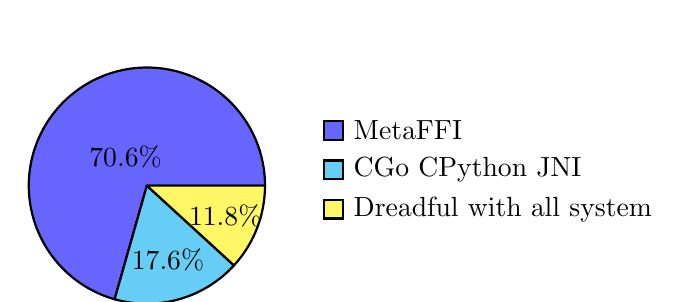
\begin{tikzpicture}
        \pie[
            text=legend,
            radius=1.5,
            after number = \%,
            legend/.style={at={(1.2,0)}, anchor=west},
        ]{
            70.6/MetaFFI,
            17.6/CGo CPython JNI,
            11.8/Dreadful with all system
        }
        \end{tikzpicture}
        \caption{Ease of Finding Bugs}
        \label{fig:bugs}
    \end{subfigure}
    \hfill
    \begin{subfigure}[b]{0.48\textwidth}
        \centering
        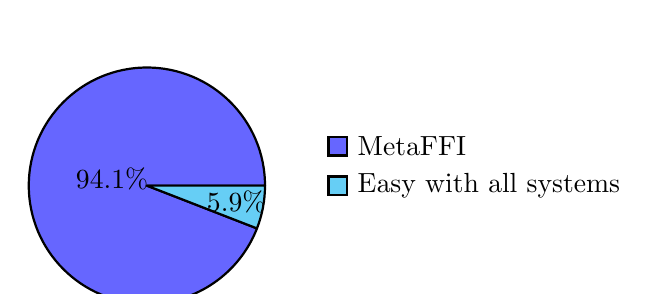
\begin{tikzpicture}
        \pie[
            text=legend,
            radius=1.5,
            after number = \%,
            legend/.style={at={(1.2,0)}, anchor=west},
        ]{
            94.1/MetaFFI,
            5.9/Easy with all systems
        }
        \end{tikzpicture}
        \caption{Ease of Making Changes in Code}
        \label{fig:changes}
    \end{subfigure}

    \vspace{1cm} % Add space between rows

    \begin{subfigure}[b]{0.48\textwidth}
        \centering
        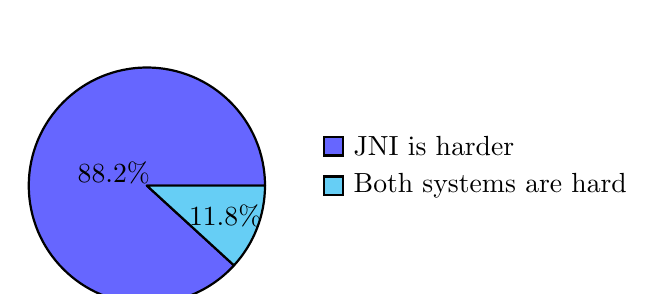
\begin{tikzpicture}
        \pie[
            text=legend,
            radius=1.5,
            after number = \%,
            legend/.style={at={(1.2,0)}, anchor=west},
        ]{
            88.2/JNI is harder,
            11.8/Both systems are hard
        }
        \end{tikzpicture}
        \caption{Comparing MetaFFI and JNI API}
        \label{fig:jni}
    \end{subfigure}
    \hfill
    \begin{subfigure}[b]{0.48\textwidth}
        \centering
        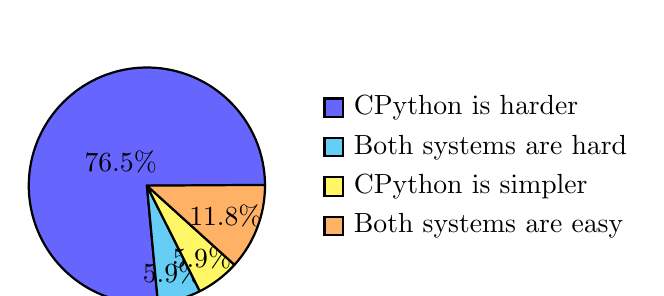
\begin{tikzpicture}
        \pie[
            text=legend,
            radius=1.5,
            after number = \%,
            legend/.style={at={(1.2,0)}, anchor=west},
        ]{
            76.5/CPython is harder,
            5.9/Both systems are hard,
            5.9/CPython is simpler,
            11.8/Both systems are easy
        }
        \end{tikzpicture}
        \caption{Comparing MetaFFI and CPython API}
        \label{fig:cpython}
    \end{subfigure}

    \vspace{1cm} % Add space between rows

    \begin{subfigure}[b]{0.48\textwidth}
        \centering
        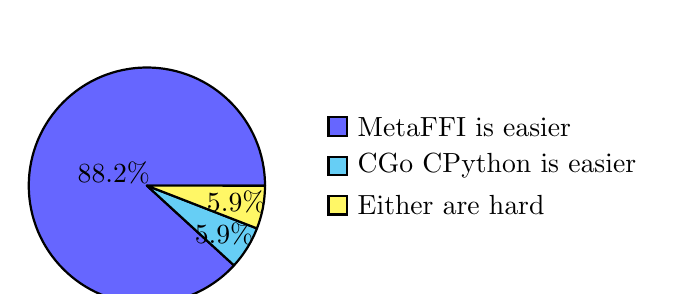
\begin{tikzpicture}
        \pie[
            text=legend,
            radius=1.5,
            after number = \%,
            legend/.style={at={(1.2,0)}, anchor=west},
        ]{
            88.2/MetaFFI is easier,
            5.9/CGo CPython is easier,
            5.9/Either are hard
        }
        \end{tikzpicture}
        \caption{Readability of Interoperability Code in Go and Python}
        \label{fig:readability}
    \end{subfigure}
    \hfill
    \begin{subfigure}[b]{0.48\textwidth}
        \centering
        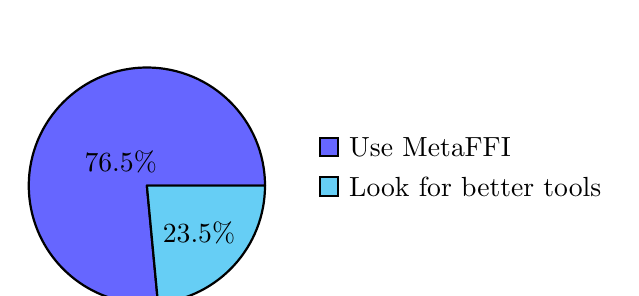
\begin{tikzpicture}
        \pie[
            text=legend,
            radius=1.5,
            after number = \%,
            legend/.style={at={(1.2,0)}, anchor=west},
        ]{
            76.5/Use MetaFFI,
            23.5/Look for better tools
        }
        \end{tikzpicture}
        \caption{Future Use of MetaFFI}
        \label{fig:future}
    \end{subfigure}
\caption{Survey Results}
\label{fig:survey}
\end{figure}

The results reveal significant insights into the practical application and user experience of the MetaFFI interoperability system. The majority of participants found MetaFFI to be notably more efficient in development time and user-friendly compared to traditional methods like CGo, CPython, and JNI. Specifically, 70.6\% of respondents indicated that finding bugs was easier with MetaFFI, while only 17.6\% preferred other methods, as shown in Figure~\ref{fig:bugs}. When it came to making changes in the code, a compelling 94.1\% found MetaFFI easier to use (Figure~\ref{fig:changes}). Furthermore, 88.2\% of the participants reported that JNI is harder to use than MetaFFI, and 76.5\% found CPython to be more challenging (Figures~\ref{fig:jni} and \ref{fig:cpython}, respectively). Additionally, 88.2\% of respondents believed that the code readability improved with MetaFFI (Figure~\ref{fig:readability}). For future use, 76.5\% of participants expressed a preference for MetaFFI, with only 23.5\% inclined to look for better tools (Figure~\ref{fig:future}). These findings underscore MetaFFI's potential to perform interoperability tasks, reduce development effort, and enhance overall code maintainability.

\textbf{Interoperability effort compared to overall workshop:}

The survey also included questions regarding the effort, in percentage, that students estimated they spent on coding with and without MetaFFI during the workshop. The specific questions were: 
\textit{If the whole workshop is 100\%, how much effort, in percentage, do you estimate you have spent on coding with MetaFFI to interoperate Go with Python and Java?} and \textit{If the whole workshop is 100\%, how much effort, in percentage, do you estimate you have spent on coding without MetaFFI (i.e., CGO/CPython/JNI) to interoperate Go with Python and Java?}

The responses to the first question indicated that the average effort spent coding with MetaFFI was 14\%, with a median of 10\%. In contrast, the responses to the second question revealed that the average effort spent coding without MetaFFI was significantly higher, at 32\%, with a median of 35\%. These results suggest that students found coding with MetaFFI to be more efficient and less time-consuming than using traditional methods for interoperability.

The substantial reduction in effort required when using MetaFFI underscores its effectiveness in simplifying the process of integrating different programming languages. By reducing the time and effort needed for programming language interoperability, MetaFFI allows developers to focus more on other critical aspects of their projects. This efficiency gain highlights MetaFFI's potential to enhance productivity and streamline development workflows in multi-PL environments.



\subsection{Experiment and Survey Conclusion}
The survey conducted during the distributed systems workshop provides valuable insights into the practical application of MetaFFI for interoperability of the programming language. The results indicate that MetaFFI significantly reduces the effort required for interoperability tasks, improves code readability, and is generally preferred by students over traditional methods involving CGo, JNI, and CPython.

The students reported a substantial decrease in the time and effort required to implement interoperability using MetaFFI compared to traditional methods. As one student mentioned, "I think it is very easy to use and pretty straightforward. The only thing I think was missing for me is a short readme file or some documentation about the module. I think it would've made it more user-friendly and helped me find my mistakes. But overall, it really simplified the work."

Most of the students found MetaFFI easier to use both to identify bugs and to make code changes. However, some feedback highlighted the challenges related to bug identification due to a lack of understanding of MetaFFI's inner workings. One student noted, "The concept of MetaFFI is simple and easy to use, but when we had bugs, it was hard to identify what the bug actually is because we didn't understand how MetaFFI works, maybe a documentation would have helped."

The feedback also emphasized the practical benefits of MetaFFI in comparison to traditional methods: "When I encountered errors in my code that stemmed from using MetaFFI, the problems were always just Java errors and nothing to do with interoperability. ... Working with MetaFFI was a breeze and made me only focus on issues/bugs in the implementation of the Java/Python code. It provided a perfect layer of abstraction without hiding away a lot of customization details of certain languages. The API and the syntax it provided were easy to understand and work with."

Also, one group indicated they added more methods to the Chord implementation and called them from Go using MetaFFI.

Overall, the findings suggest that MetaFFI offers a good approach for simplifying and improving the process of programming language interoperability. One student summarized their experience by saying, "MetaFFI was much easier to use, especially when it replaced JNI."

The survey emphasizes the importance of improving the documentation of MetaFFI, which currently lacks.


\section{Conclusions}


\bibliography{zotero}

\end{document}
